% \iffalse meta-comment
% !TeX program  = xelatex
% !TeX encoding = UTF-8
% 
% Copyright (C) 2015--2019 by Stick Cui <Stick_Cui@163.com>
% 
% This file may be distributed and/or modified under the
% conditions of the LaTeX Project Public License, either version 1.3c
% of this license or (at your option) any later version.
% The latest version of this license is in:
%
% http://www.latex-project.org/lppl.txt
%
% and version 1.3c or later is part of all distributions of LaTeX
% version 2008/05/04 or later.

%<*internal>
\def\nameofplainTeX{plain}
\ifx\fmtname\nameofplainTeX\else
  \expandafter\begingroup
\fi
%</internal>
%<*install>

\input docstrip
\keepsilent
\askforoverwritefalse
\preamble

This is a generated file.

Copyright (C) 2015--\the\year by Stick Cui <Stick_Cui@163.com>

This file may be distributed and/or modified under the
conditions of the LaTeX Project Public License, either version 1.3c
of this license or (at your option) any later version.
The latest version of this license is in:

http://www.latex-project.org/lppl.txt

and version 1.3c or later is part of all distributions of LaTeX
version 2008/05/04 or later.

To produce the documentation run the original source files ending with `.dtx'
through LaTeX.

\endpreamble
\postamble

This package consists of the file  XDUthesis.dtx,
             and the derived files XDUthesis.cls,
                                   XDUthesis.cfg.        

\endpostamble

\usedir{tex/latex/XDUthesis}
\generate
  {
    \file{XDUthesis.cls}{\from{\jobname.dtx}{cls}}
    \file{XDUthesis.cfg}{\from{\jobname.dtx}{cfg}}
  }

\Msg{***********************************************************}
\Msg{*}
\Msg{* To finish the installation you have to move the following}
\Msg{* files into a directory searched by TeX:}
\Msg{*}
\Msg{* The recommended directory is TEXMF/tex/latex/XDUthesis}
\Msg{*}
\Msg{* \space\space XDUthesis.cls}
\Msg{* \space\space XDUthesis.cfg}
\Msg{*}
\Msg{* To produce the documentation run the files ending with}
\Msg{* `.dtx' through LaTeX.}
\Msg{*}
\Msg{* Happy TeXing!}
\Msg{***********************************************************}

%</install>
%<install>\endbatchfile
%<*internal>

\usedir{tex/latex/XDUthesis}
\generate
  {
    \file{\jobname.ins}{\from{\jobname.dtx}{install}}
  }
\nopreamble\nopostamble

\ifx\fmtname\nameofplainTeX
  \expandafter\endbatchfile
\else
  \expandafter\endgroup
\fi
%</internal>}
%<cls>\NeedsTeXFormat{LaTeX2e}
%<cls>\ProvidesClass{XDUthesis}
%<cfg>\ProvidesFile{XDUthesis.cfg}
%<cls|cfg>[2019/04/17 0.1.8 Xidian University Thesis Template]
%<*driver>
\ProvidesFile{XDUthesis.dtx}[2019/04/17 0.1.8 Xidian University Thesis Template]
\documentclass[10pt]{ltxdoc}

\usepackage[left=4cm,right=3cm,top=3cm,bottom=2cm]{geometry}
\usepackage[SlantFont,BoldFont,CJKchecksingle]{xeCJK}
\usepackage{indentfirst}
\setlength{\parindent}{2em}
\usepackage[toc,page,title,titletoc,header]{appendix}
\usepackage{longtable,multirow,hhline,tabularx,array,makecell,booktabs,diagbox}
\usepackage{metalogo,xcolor}
\usepackage{pst-barcode}%
\usepackage{fancyvrb,CJKfntef}
\usepackage[bookmarks=true,%
    linkcolor=black,%
    citecolor=black,%
    unicode=true,%
    colorlinks=true,%
    pdfborder=001,%
    urlcolor=black,
    bookmarksnumbered=true%
]{hyperref}
\def\XDUthesis{X\kern -.1667em\lower .5ex\hbox {D}\kern -.125emU\textit{thesis}{}}

\renewcommand{\abstractname}{摘\quad 要}
\renewcommand{\contentsname}{目\quad 录}
\renewcommand{\appendixname}{附\quad 录}
\renewcommand{\figurename}{图}
\renewcommand{\tablename}{表}
\renewcommand\refname{参考文献}
\renewcommand{\indexname}{索\quad 引}
\def\pkg#1{\texttt{#1}}

\usepackage{fancyhdr}
\setlength{\headheight}{15pt}
\fancyhf{}
\fancyhead[L]{\leftmark}
\fancyhead[R]{\thepage}
\renewcommand\headrulewidth{0.5pt}
\renewcommand{\footrulewidth}{0pt}
\fancypagestyle{headings}{
\fancyhf{}
\fancyhead[C]{\contentsname}
\renewcommand{\headrulewidth}{0.5pt}
\renewcommand{\footrulewidth}{0pt}}
\pagestyle{fancy}

\newfontfamily\CouNew{Courier New}
\def\codebasicfont{\fontfamily{Courier New}\selectfont}

\DefineVerbatimEnvironment{example}{Verbatim}%
  {frame=single,framerule=0.3mm,rulecolor=\color{red!70!green!20!blue!20},%
   fillcolor=\color{red!75!green!50!blue!15},framesep=0.5mm,baselinestretch=1.2,%
   fontsize=\small,gobble=1}
\DefineVerbatimEnvironment{shell}{Verbatim}%
  {frame=single,framerule=0.3mm,rulecolor=\color{red!0!green!25!blue!51},%
   fillcolor=\color{red!20!green!20!blue!50},framesep=0.5mm,fontsize=\small,gobble=1}

\EnableCrossrefs
\CodelineIndex
\RecordChanges

\begin{document}
  \DocInput{\jobname.dtx}
  \PrintChanges
  \PrintIndex
\end{document}
%</driver>
% \fi
%
% \CheckSum{977}
% \CharacterTable
%  {Upper-case    \A\B\C\D\E\F\G\H\I\J\K\L\M\N\O\P\Q\R\S\T\U\V\W\X\Y\Z
%   Lower-case    \a\b\c\d\e\f\g\h\i\j\k\l\m\n\o\p\q\r\s\t\u\v\w\x\y\z
%   Digits        \0\1\2\3\4\5\6\7\8\9
%   Exclamation   \!     Double quote  \"     Hash (number) \#
%   Dollar        \$     Percent       \%     Ampersand     \&
%   Acute accent  \'     Left paren    \(     Right paren   \)
%   Asterisk      \*     Plus          \+     Comma         \,
%   Minus         \-     Point         \.     Solidus       \/
%   Colon         \:     Semicolon     \;     Less than     \<
%   Equals        \=     Greater than  \>     Question mark \?
%   Commercial at \@     Left bracket  \[     Backslash     \\
%   Right bracket \]     Circumflex    \^     Underscore    \_
%   Grave accent  \`     Left brace    \{     Vertical bar  \|
%   Right brace   \}     Tilde         \~}
%
% \GetFileInfo{\jobname.dtx}
%
% \changes{v0.1}{2015/12/02}{finish bachelor thesis}
%
% \DoNotIndex{\begin,\end,\begingroup,\endgroup}
% \DoNotIndex{\ifx,\ifdim,\ifnum,\ifcase,\else,\or,\fi}
% \DoNotIndex{\let,\def,\xdef,\newcommand,\renewcommand}
% \DoNotIndex{\expandafter,\csname,\endcsname,\relax,\protect}
% \DoNotIndex{\Huge,\huge,\LARGE,\Large,\large,\normalsize}
% \DoNotIndex{\small,\footnotesize,\scriptsize,\tiny}
% \DoNotIndex{\normalfont,\bfseries,\slshape,\interlinepenalty}
% \DoNotIndex{\hfil,\par,\hskip,\vskip,\vspace,\quad}
% \DoNotIndex{\centering,\raggedright}
% \DoNotIndex{\c@secnumdepth,\@startsection,\@setfontsize}
% \DoNotIndex{\ ,\@plus,\@minus,\p@,\z@,\@m,\@M,\@ne,\m@ne}
% \DoNotIndex{\@@par,\DeclareOperation,\RequirePackage,\LoadClass}
% \DoNotIndex{\AtBeginDocument,\AtEndDocument}
%
% \IndexPrologue{\section*{索~~~~引}}
% \GlossaryPrologue{\section*{修改记录}}
%
% \title{\XDUthesis 西安电子科技大学本科生毕业设计论文模板\thanks{Xidian University \LaTeX{} Thesis Template}}
% \author{崔元顺\thanks{西安电子科技大学数学与统计学院2012级本科生}}
% \date{v\fileversion\ (\filedate)}
% 
% \maketitle\thispagestyle{empty}
% \begin{abstract}
%  本模板旨在减轻排版工作量,使得学生专注于论文质量本身。鉴于初级阶段,仅包含本科毕业设计论文% 部分。
% \end{abstract}
% 
% \vspace*{2em}
% \def\abstractname{免责声明}
% \begin{abstract}
% \noindent
%  \begin{enumerate}
%  \item 本模板的前期制作部分参考\href{http://www.ctan.org/pkg/thuthesis}{清华大学学位论文模板},且遵守 \LaTeX{} Project Public  License,使用前请认真阅读协议内容。
%  \item 本模板的制作过程参考\href{http://jwc.xidian.edu.cn}{西安电子科技大学教务处}发布的《本科生毕业设计(论文)工作手册》,仅供\href{http://www.xidian.edu.cn}{西安电子科技大学}本科生撰写毕业设计论文使用。
%  \item 本模板为作者参考官方工作手册要求个人制作,使用仅供参考,任何由于使用本模板而引起的论 文格式审查问题均与本模板作者无关。
%  \item 任何个人或组织以本模板为基础进行修改、扩展而生成的新的专用模板,请严格遵守 \LaTeX{}  Project Public License 协议。由于违犯协议而引起的任何纠纷争端均与本模板作者无关。
%  \end{enumerate}
% \end{abstract}
% 
% \clearpage
% \thispagestyle{headings}
% \begin{multicols}{2}[
%   \setlength{\columnseprule}{.4pt}
%   \setlength{\columnsep}{18pt}]
%   \tableofcontents
% \end{multicols}
% \clearpage
% \pagenumbering{arabic}
% 
% \section{模板介绍}
% \XDUthesis{} 是专为西安电子科技大学本科毕业生而写的\LaTeX{} 模板。
% 
% 在此,有关本模板的使用方法以及相关注意事项,将尽可能地在本文中叙述;
% 遵守本模板中的一些规则,将大大减少论文排版时间。\footnote{因使用者个人修改或未遵守本模板规范,而造成的论文版式不规范,与\XDUthesis{} 模板作者无关。}
% 
% 在 \ref{SubSec:HowToMake} 小节,介绍了如何去编译文档,对于没接触过\BibTeX{} 的用户,在 \ref{SubSec:ForBibTeX} 小节还补充介绍了配合\BibTeX{}编译文档的原理。除了本模板自带的使用样例,本文档的 \ref{SubSec:ThesisSample} 小节中还给出了一个十分简洁的小样例,供大家入门学习。
% 
% \section{模板信息}
% \subsection{模板组成}
% \begin{longtable}[c]{l|m{9cm}}
% \caption{\XDUthesis{} 模板主要文件(夹)及功能介绍}\label{Tab:XDUthesisALL}\\
% \hline
% \textbf{文件(夹)} & \textbf{功能描述}\\\hline\hline
% \endfirsthead
% \multicolumn{2}{l}{(续表)}\\
% \hline
% \textbf{文件(夹)} & \textbf{功能描述}\\\hline\hline
% \endhead
% \hline
% \multicolumn{2}{c}{接下页$\cdots$}
% \endfoot
% \hline
% \endlastfoot
% 
% XDUthesis.dtx & 模板主文件\\
% XDUthesis.cls & 模板文档类文件(需生成)\\
% XDUthesis.cfg & 模板配置文件(需生成)\\
% Demo.tex & 模板示例拆分文档的主文档\footnote{将整个论文拆分为几个部分,汇总在本文件}\\
% gbt7714-plain.bst & 参考文献样式文件(排序)\\
% gbt7714-unsrt.bst & 参考文献样式文件(不排序)\\
% ThesisFiles/ & 模板示例拆分文档的存储目录\\
% Abstract.tex & 模板示例拆分文档的摘要部分(存放于ThesisFiles)\\
% Chapters.tex & 模板示例拆分文档的主要章节部分(存放于ThesisFiles)\footnote{可根据需要再行修改或拆分,添加到Main.tex中;}\\
% Thanks.tex & 模板示例拆分文档的致谢部分(存放于ThesisFiles)\\
% Appendix.tex & 模板示例拆分文档的附录部分(存放于ThesisFiles)\\
% RefFile.bib & 参考文献库示例文档(存放于ThesisFiles)\\
% Code/ & 源代码文件夹,存放各种程序源代码(附录用)\\
% Figure/ & 图片文件夹,存放各种文章中用到的图\footnote{\textbf{\color{red}目录里面的logo.pdf和xidian.pdf勿动,模板封面要用!!!}}\\
% make.bat & 生成模板类、说明文档等Windows脚本\\
% \textbf{XDUthesis.pdf} & 用户手册(本文档,需生成)\\
% \end{longtable}
% \textbf{注:}使用前,请仔细阅读\textbf{XDUthesis.pdf},即本文档。
% 
% \subsection{使用前的准备}
% 
% \XDUthesis{} 模板基于ctex中文套件中的ctexbook (2016/02/02 v2.3)而写,因此用户需要确保安装了此版本(或更新)的ctex套件,如没有安装可前往\textbf{CTAN: \url{http://www.ctan.org}} 或者前往\textbf{GitHub(CTeX-org): \url{https://github.com/CTeX-org/ctex-kit/releases}} 下载。
% 
% 除以上,本模板还依赖以下宏包:
% 
% \begin{table}[ht]
% \centering
% \caption{\XDUthesis{} 依赖宏包}\label{Tab:pkg}
% \begin{tabular}{*{6}l}
% \hline
% \pkg{ifxetex} & \pkg{xcolor} & \pkg{fontenc} & \pkg{amsmath} & \pkg{amssymb} & \pkg{graphicx}\\
% \pkg{ntheorem} & \pkg{natbib} & \pkg{appendix} & \pkg{listings} & \pkg{longtable} & \pkg{multirow}\\
% \pkg{hhline} & \pkg{tabularx} & \pkg{array} & \pkg{makecell} & \pkg{colortbl} & \pkg{booktabs}\\
% \pkg{hyperref} & \pkg{geometry} & \pkg{fancyhdr} & \pkg{CJKfntef} & \pkg{subcaption} & \pkg{setspace}\\
% \pkg{blindtext} & \pkg{pifont} &&&&\\
% \hline
% \end{tabular}
% \end{table}
% 表 \ref{Tab:pkg} 中宏包,常见的\TeX{} 发行版都会集成好,比如作者本人开发时使用的TeXLive2015既涵盖了ctex中文套件,也包含了表 \ref{Tab:pkg} 中的所有宏包。 如使用的其他系统\footnote{比如CTeX中文小组维护的CTeX 2.9版本,里面集成的宏包都比较老,需要手动下载更新。一般用户根本不知道如何去做。因此作者推荐TeXLive2015.}缺少表 \ref{Tab:pkg} 中宏包任几个,可去往\textbf{CTAN: \url{http://www.ctan.org}} 下载。
% 
% \section{如何提问}
% 这一节本想只介绍如何联系作者本人解决问题呢,后来想想,肯定忙不过来就算了。还是将 \XDUthesis{} 和 \LaTeX{} 本身的疑问分开来叙述比较妥当。
% \subsection[关于XDUthesis模板的疑问]{关于\XDUthesis{} 模板的疑问}
% 使用本模板的过程中,如有任何关于本模板的疑问或是不懂之处可通过以下渠道联系作者本人:
% \begin{itemize}
% \item 新浪微博:\href{http://weibo.com/StickCui}{I-am-13}. 或手机扫描以下二维码私信作者。
% 
% \begin{center}
% \begin{pspicture}(1.5in,1.5in)
% \psbarcode{http://weibo.cn/qr/userinfo?uid=3024285285}{includetext guardwhitespace width=1.5 includetext guardwhitespace height=1.5 eclevel=H}{qrcode}
% \end{pspicture}
% \end{center}
% 
% \item 邮箱:\href{mailto:Stick\_Cui@163.com}{Stick\_Cui@163.com}
% \end{itemize}
% 就说上面两个吧,知道作者QQ的童鞋还可以直接私聊。
% 
% \subsection[关于LaTeX的疑问]{关于\LaTeX{} 的疑问}
% 
% 使用\LaTeX{} 排版写作的过程不是一帆风顺的。一个完整的文章往往需要几十上百次,有的甚至上千次的编译调试才能完成。
% 
% 中间碰到的任何问题都有可能把写作人绊住。因为不是所有问题都能单独去解决的,这时就需要去上网检索解决方案,但不是所有检索到的解决方案都是适用的,有些可能已过时。这就需要写作人一一辨别、尝试。
% 
% 在这里作者给大家提几条网上检索的工具:
% \begin{itemize}
% \item 谷歌搜索: \href{https://www.google.com}{https://www.google.com}
% 
% 这个一般国内用户无法使用,原因不提。但无疑它是最好的,有能力科学上网的用户可以选择它,如何检索不提了。
% 
% \item 知乎: \href{http://www.zhihu.com}{http://www.zhihu.com}
% 
% 知乎里面的\textbf{\LaTeX{}} 话题以及\textbf{\LaTeX{} 排版与设计}话题下有很多关于排版难题以及技巧的高质量答案。这方面领域的牛人有:\href{http://www.zhihu.com/people/qinglee}{李清}、\href{http://www.zhihu.com/people/li-a-ling}{李阿玲}\footnote{本名:马起园,男,pTeX-ng开发者}、\href{http://www.zhihu.com/people/liu-haiyang}{刘海洋}、\href{http://www.zhihu.com/people/LiamHuang}{孟晨}等。
% 
% \item 百度:这个不给链接了,也不多解释了。
% \end{itemize}
% 
% \section{使用模板}
% \subsection{如何编译}\label{SubSec:HowToMake}
% 首先,要感谢一下\href{http://www.zhihu.com/people/qinglee}{李清}等前辈们的贡献,基于ctex中文套件开发,省了不少功夫。\footnote{减少了对不同编译引擎的处理工作。}
% 
% 本模板支持的编译命令有:\textbf{xelatex}, \textbf{pdflatex}, \textbf{latexmk}.
% 作者在这里推荐使用\textbf{xelatex} 或者 \textbf{latexmk} + \textbf{xelatex}.原因见后文。
% 
% \subsubsection{pdflatex命令}
% 对于一些\LaTeX{} 初入门者,就我身边的人而言,大多数人喜欢用各种编辑器默认的\textbf{pdflatex} 去编译文件。所以,首先说一下\textbf{pdflatex} 的编译方法。以编译Template.tex为例。
% 
% \begin{enumerate}
% \item \textbf{命令行}
% 
% \begin{shell}
% pdflatex Demo
% bibtex Demo
% pdflatex Demo
% pdflatex Demo
% \end{shell}
% 
% \item \textbf{编辑器}
% 
% 编译顺序同上,在编辑器里
% 
% 点击\textbf{PDFLaTeX} 编译按钮编译一次;
% 
% 点击\textbf{BibTeX} 编译按钮编译一次;
% 
% 再次点击\textbf{PDFLaTeX} 编译按钮编译两次;
% \end{enumerate}
% 
% PDF\LaTeX{} 引擎不支持eps矢量图的插入,需要先转为pdf文件才可。\footnote{不用担心,使用TeXLive2010及之后版本,会自动将其转为pdf.}且pdf使用的CJK方式处理的中文有些蹩脚,不是很好,尤其是中英文之间的空格以及标点符号的处理。故此不推荐使用此方式编译文档。
% 
% \subsubsection{xelatex命令}
% 
% \begin{enumerate}
% \item \textbf{命令行}
% 
% \begin{shell}
% xelatex Demo
% bibtex Demo
% xelatex Demo
% xelatex Demo
% \end{shell}
% 
% \item \textbf{编辑器}
% 
% 编译顺序同上,在编辑器里
% 
% 点击\textbf{XeLaTeX} 编译按钮编译一次;
% 
% 点击\textbf{BibTeX} 编译按钮编译一次;
% 
% 再次点击\textbf{XeLaTeX} 编译按钮编译两次;
% \end{enumerate}
% 
% 此方式对中文处理的很好,推荐此方式。
% 
% \subsubsection{latexmk + xelatex命令}
% 
% \textbf{latexmk} 命令能够自动编译\LaTeX{} 文档,并可以支持不同工具链接来生成;它会自动运行多次工具直到交叉引用都被解决。也就是说,它只需要运行一遍就行了。
% 下面是\textbf{latexmk} 命令结合\textbf{xelatex} 命令编译的示例:
% 
% \begin{shell}
% latexmk -xelatex Demo
% \end{shell}
% 
% 此处,就不说编辑器里的了,不同的编辑器需要不同的配置。
% 
% 以上。
% 
% \subsection[补充介绍BibTeX]{补充介绍\BibTeX}\label{SubSec:ForBibTeX}
% \BibTeX{} 是\LaTeX{} 自动化工具里面一个强大的参考文献管理工具,依据用户指定的参考文献样式,它能够出色完成参考文献的排序以及生成。
% 
% 参考文献样式有命令:\verb=\bibliographystyle{}= 控制;命令:\verb=\bibliography{}= 将参考文献库通过处理后写入正文。以下以\textbf{xelatex} 命令编译Template.tex文件为例,进行详细描述该过程。
% 
% \begin{enumerate}
% \item 首次运行 \verb=xelatex Template.tex= ,程序执行到 \verb=\bibliography{RefFile}= 时,会进行判断有无指定的Template.bbl文件,有则加载进来;紧接着无论有无Template.bbl 文件,都会把 \verb=\cite{}= 命令产生的文档引用信息、\verb=\bibliography{RefFile}= 指定的RefFile.bib数据库名字以及\\ \verb=\bibliographystyle{XDUbib}= 指定的XDUbib.bst文献格式名都写入Template.aux辅助文件;此时生成的PDF 参考文献只有标题,没有列表。
% 
% \item 运行 \verb=bibtex Template.aux= ,按照其中记录的引用、文献信息,从RefFile.bib数据库中提取出来排版参考文献列表(\LaTeX{}代码),写入Template.bbl文件。
% 
% \item 再次运行 \verb=xelatex Template.tex= ,读入对应Template.bbl,生成有参考文献列表的PDF,同时将 \verb=\cite{}= 产生的引用信息再次写入Template.aux辅助文件;
% 
% \item 最后一次运行 \verb=xelatex Template.tex= ,读入对应Template.bbl,在指定位置生成参考文献列表,读入上步生成的Template.aux辅助文件,在引用处生成正确的引用编号信息,得到有正确文献列表和引用的PDF文件。
% \end{enumerate}
% 
% \noindent 以上就是一般需要编译四次的原因。
% 
% \subsection{一个简单的使用样例}\label{SubSec:ThesisSample}
% 以下,给出一个使用本模板写作的样例,并在注释信息中说明每一部分的作用。
% 
% \begin{example}
% \documentclass[WordOneHalf]{XDUthesis}
% \title{基于ctex套件的模板制作过程}
% \author{崔元顺}
% \date{2015年12月02日}%如果是今天可以是\today或省略不写
% %题目拆分:用于封面
% %如果论文题目长度<=11中文字符只需填此项即可B项空着
% \septitleA{基于ctex套件的模板}
% %如果论文题目长度>11中文字符, 建议拆分为10+x or 11+x 将剩余x个字符填在此处。
% \septitleB{制作过程}
% \class{0712**}%班级号
% \schoolnumber{0712****}%学号
% \major{统计学}%专业
% \school{数学与统计学院}%学院
% \supervisor{崔元顺}%指导老师
% 
% \begin{document}
% 
% % 中文摘要
% \begin{abstract}
%   摘要测试,朕要测试一下\textit{斜体}
%   模板名字\XDUthesis~
% \end{abstract}
% \keywords{朕, 模板}中文关键词,这里注意用半角字符,分隔
% 
% % 英文摘要
% \begin{enabstract}
%   Abstract test. I want to test \textit{italic}
%   The template's name is \XDUthesis~
% \end{enabstract}
% \enkeywords{I, template} %英文关键词
% 
% % 往PDF属性里面写下关键词信息,勿动
% \makeatletter
% \XDU@setpdf@keywords
% \makeatother
% 
% % 显示封面、诚信声明书、摘要以及目录
% \maketitle
% 
% % 正文内容
% \chapter{引言}
% 
% balabala
% 
% \chapter{结束语}
% 
% \begin{thanksfor}
%  这里是致谢部分。感谢崔元顺。
% 
%  恩,不客气。
% \end{thanksfor}
% 
% %参考文献
% \phantomsection%生成该页的链接
% \addcontentsline{toc}{chapter}{\bibname}
% \bibliographystyle{XDUbib}
% \bibliography{RefFile}%在正文中必须引用,才能显示对应的参考文献
% 
% % 附录部分
% \appendix
% % 附录A
% \chapter{数据}
% 这里是附录的数据部分
% 
% \end{document}
% \end{example}
% 
% \subsection{关于配置文件}\label{SubSec:aboutCFG}
% 
% \textbf{XDUthesis.cfg} 是本模板的配置文件,关于论文中的相关标题名称,配色,相关关键词名称,摘要关键词分隔符,定理类环境的定义,字体等相关设置,均存放于此文件。
% 
% 关于上述相关配置,哪些可以修改,哪些禁止修改,里面的注释中均有说明。再次声明:个人因需要修改、删除或添加的配置信息,如发生论文排版不合格等意外,与本模板作者无关。
% 
% \subsection{字体配置}
% 根据西安电子科技大学教务处印发的《本科生毕业设计(论文)工作手册》规定,主要用的字体有:中文--黑体,宋体;英文--Times News Roman.
% 
% 本模板开发之时是基于Windows 10上的TeXLive2015,默认字体刚好符合;作者由于经济等原因并未在其他操作系统平台或其他\TeX{} 发行版中进行测试。如在使用中发现字体不符合学校要求字体,可通过以下命令查找到正确字体,并参考《C\TeX{} 套件手册》在 \ref{SubSec:aboutCFG} 小节中提到的配置文件里面进行修改:
% 
% \begin{shell}
% fc-list :lang=zh file family style > zhfonts.txt
% \end{shell}
% 
% \noindent\textbf{注:}以上命令,会在终端当前状态所处的文件夹下生成zhfonts.txt文件,里面列出了当前系统下已安装的所有中文字体。
% 
% \subsection{命令}
% \subsubsection{基础命令}
% 鉴于本文档基于的是ctex套件,故而,作者先叙述ctexbook中的基础命令。
% \begin{enumerate}
% 
% \item \textbf{字号}
% 
% \begin{table}[ht]
% \centering
% \caption{基础字号命令}\label{Tab:basicFontSize}
% \begin{tabular}{l c | l c}
% \hline
% 字体命令 & 字号 & 字体命令 & 字号\\
% \hline
% \verb=\tine= & 小六 & \verb=\large= & 小三\\
% \verb=\scriptsize= & 六号 & \verb=\Large= & 小二\\
% \verb=\footnotesize= & 小五 & \verb=\LARGE= & 二号\\
% \verb=\small= & 五号 & \verb=\huge= & 小一\\
% \verb=\normalsize= & 小四 & \verb=\Huge= & 一号\\
% \hline
% \end{tabular}
% \end{table}
% 
% 除了表 \ref{Tab:basicFontSize} 中的基础字号命令外,ctex套件还提供了 \verb=\zihao{<字号>}= 命令用以修改或设置字号,具体设置详情见表 \ref{Tab:setFontSize}.
% 
% \begin{table}[ht]
% \centering
% \caption{中文字号}\label{Tab:setFontSize}
% \begin{tabular}{c c l}
% \hline
% <字号> & 大小(bp) & 意义\\
% \hline
% 0 & 42 & 初号\\
% -0 & 36 & 小初号\\
% 1 & 26 & 一号\\
% -1 & 24 & 小一号\\
% 2 & 22 & 二号\\
% -2 & 18 & 小二号\\
% 3 & 16 & 三号\\
% -3 & 15 & 小三号\\
% 4 & 14 & 四号\\
% -4 & 12 & 小四号\\
% 5 & 10.5 & 五号\\
% -5 & 9 & 小五号\\
% 6 & 7.5 & 六号\\
% -6 & 6.5 & 小六号\\
% 7 & 5.5 & 七号\\
% 8 & 5 & 八号\\
% \hline
% \end{tabular}
% \end{table}
% 
% \item \textbf{字体选择}
% 
% ctex套件预定义了一些常用字体的快捷调用命令,详情如下:
% 
% \begin{itemize}
% 
% \item[\textbf{\textbackslash songti}] 宋体,CJK等价命令\verb=\CJKfamily{zhsong}=;
% \item[\textbf{\textbackslash heiti}] 黑体,CJK等价命令\verb=\CJKfamily{zhhei}=;
% \item[\textbf{\textbackslash fangsong}] 仿宋,CJK等价命令\verb=\CJKfamily{zhfs}=;
% \item[\textbf{\textbackslash kaishu}] 楷书,CJK等价命令\verb=\CJKfamily{zhkai}=;
% 
% 其中 \verb=\fangsong= 在ubuntu字库中没有定义。在windows和founder字库中,还有 \verb=\lishu= % 和 \verb=\youyuan=。
% 
% \item[\textbf{\textbackslash lishu}] 隶书,CJK等价命令\verb=\CJKfamily{zhli}=;Fandol字库中没有定义。
% \item[\textbf{\textbackslash youyuan}] 幼圆,CJK等价命令\verb=\CJKfamily{zhyou}=;Fandol字库中没有定义。
% 
% 在windowsnew字库中,还有 \verb=\yahei=。
% 
% \item[\textbf{\textbackslash yahei}] 微软雅黑,CJK等价命令\verb=\CJKfamily{zhyahei}=;Fandol字库中没有定义。
% \end{itemize}
% 
% \item \textbf{下划线}
% 
% 借助\pkg{CJKfntef}宏包,拥有了很多样式的下划线种类。以下是常用到的五类。\footnote{为了展示% 效果,没有去修改颜色,模板里均为黑色。}
% \begin{itemize}
%   \item[\textbf{\textbackslash CJKunderline\{\}}] 下划线:\CJKunderline{下划线}
%   \item[\textbf{\textbackslash CJKunderdblline\{\}}] 双下划线:\CJKunderdblline{双下划线}
%   \item[\textbf{\textbackslash CJKunderwave\{\}}] 波浪线:\CJKunderwave{波浪线}
%   \item[\textbf{\textbackslash CJKunderdot\{\}}] 加点着重符号:\CJKunderdot{加点着重符号}
%   \item[\textbf{\textbackslash CJKsout\{\}}] 删除线:\CJKsout{删除线}
% \end{itemize}
% 
% \item \textbf{其他}
% 
% 在图表的浮动环境里,支持使用 \verb=\subcaptionbox{<子图(表)标题>}{<子图(表)内容>}= 命令去插入子图或者子表。
% 
% 将一个计数器显示为中文数字可以使用命令 \verb=\chinese{<counter>}=,将一个普通数字(整数、浮点数、分数)可以使用 \verb=\zhnumber{<number>}=,将一串阿拉伯数字转换为中文字符串可以使用 \verb=\zhdigits{<number>}=,等等。其他详见《C\TeX{} 套件手册》。\footnote{以TeXLive2015为例,命令行终端运行 \textbf{texdoc ctex} 即可。}
% 
% \end{enumerate}
% 
% \subsubsection{可选参数}
% 使用时,在模板开始时,即\verb=\documentclass[para]{XDUthesis}=,其中para可以是以下一个或多个:
% \begin{itemize}
%  \item \textbf{Fandol}:使用Fandol字库,此时无幼圆、隶书、微软雅黑字体定义命令,如需使用,请自行设置
%  \item \textbf{nologo}:封面不使用学校的Logo
%  \item \textbf{WordOneHalf}:设置行距为Word版的1.5倍行距
% \end{itemize}
% 
% \subsubsection{控制命令}
% \begin{enumerate}
% 
% \item \textbf{封面页控制命令}
% 
% 以下命令均需要用在 \verb=\maketitle= 之前。
% 
% \begin{enumerate}
% \item[\textbf{\textbackslash title\{\}}] 论文标题;
% \item[\textbf{\textbackslash septitleA\{\}}] 论文标题拆分之A 部分;
% \item[\textbf{\textbackslash septitleB\{\}}] 论文标题拆分之B 部分;
% 
% 这里解释一下为什么还要将论文题目拆分。由于我校的封面部分给论文题目留了两条线,且每条线极限容纳字数为11个中文字符;因此,如果题目超过11个中文字符,有必要对论文题目拆分,如何拆分?
% 作者原本是想要自动拆分的,然而,能力有限,目前还不会。而且自动拆分如果效果不理想还是要手动,所以干脆手动吧。在 \ref{SubSec:ThesisSample} 小节的样例中给了一种解决方法,实际应用时还是要具体问题具体分析。
% 
% \item[\textbf{\textbackslash author\{\}}] 论文作者;
% \item[\textbf{\textbackslash date\{\}}] 论文写作时间or提交时间;
% \item[\textbf{\textbackslash class\{\}}] 作者班级号;
% \item[\textbf{\textbackslash schoolnumber\{\}}] 作者学号;
% \item[\textbf{\textbackslash major\{\}}] 作者专业;
% \item[\textbf{\textbackslash school\{\}}] 作者所在学院;
% \item[\textbf{\textbackslash supervisor\{\}}] 作者的论文指导老师;
% \item[\textbf{\textbackslash keywords\{\}}] 中文摘要关键词,与\textbf{abstract}环境配合使用;
% \item[\textbf{\textbackslash enkeywords\{\}}] 英文摘要关键词与\textbf{enabstract}环境配合使用;
% \end{enumerate}
% 
% \item \textbf{其他命令}
% 
% \begin{itemize}
% \item[\textbf{L{<length>}}] 表格控制参数:水平左对齐,列宽为 \verb=<length>= 指定值;
% \item[\textbf{R{<length>}}] 表格控制参数:水平右对齐,列宽为 \verb=<length>= 指定值;
% \item[\textbf{C{<length>}}] 表格控制参数:水平居中对齐,列宽为 \verb=<length>= 指定值;
% 
% \hspace*{-2em} 以下命令太长,反过来叙述。(别打我)\SaveVerb{zhuanyi}|`|
% \item[\textbf{代码文件插入}] \verb=\lstinputlisting[<para>]{<file>}=;\footnote{针对PDF\LaTeX{} 引擎,专门添加了转义字符“\,{\CouNew{\UseVerb{zhuanyi}}}\,”,用于代码中显示中文注释、字符串等。}
% 
% \verb=<file>= 是文件路径及文件名,UTF-8编码(尤其是有中文注释时)。
% 
% \verb=<para>= 可以有许多参数,最重要的是 \verb|language = ?| 问号是编程语言,具体支持的较多,可自行查阅参考文献。如果需要对源代码加标题可以使用 \verb|caption = {}| 带编号、\verb|title = {}| 不带编号。加引用标签可以使用 \verb|label = ?|。 选择不同的代码显示风格可以使用\verb|style = ?|,代码显示风格可以通过 \verb|\lstdefinestyle{<stylename>}{<style>}| 命令自定义,本模板预定义好了\verb|nonumbers| 无行号风格。
% 
% 不同参数之间以半角字符“,”分隔。
% 
% \item[\textbf{超链接}] \verb=\href{<url>}{<obj>}= : 对 \verb=<obj>= 加上超链接 \verb=<url>=;
% 
% \verb=\url{<url>}= : 在文中显示链接 \verb=<url>= 并加上超链接 \verb=<url>=;
% \end{itemize}
% 
% \end{enumerate}
% \begin{macro}{\onlinecite}
% 非上角标式参考文献引用命令。
% \end{macro}
% 
% \subsection{环境}
% 
% \subsubsection{控制环境}
% 
% \begin{itemize}
% \item[\textbf{abstract}] 中文摘要,需用在 \verb=\maketitle= 之前;
% \item[\textbf{enabstract}] 英文摘要,需用在 \verb=\maketitle= 之前;
% \item[\textbf{thanksfor}] 致谢环境,需用在指定位置即可;
% \end{itemize}
% 
% \subsubsection{数学环境}
% 主要涉及到的是定理类环境。\footnote{“借鉴”清华大学学位论文模板}
% \begin{multicols}{2}[
%   \setlength{\columnseprule}{0pt}
%   \setlength{\columnsep}{18pt}]
% \begin{itemize}
% \item[\textbf{proof}] 证明,证明定理或结论用;
% \item[\textbf{assumption}] 假设;
% \item[\textbf{definition}] 定义;
% \item[\textbf{proposition}] 命题;
% \item[\textbf{lemma}] 引理;
% \item[\textbf{theorem}] 定理;
% \item[\textbf{axiom}] 公理;
% \item[\textbf{corollary}] 推论;
% \item[\textbf{exercise}] 练习;
% \item[\textbf{example}] 例,举例用;
% \item[\textbf{remark}] 注释;
% \item[\textbf{problem}] 问题;
% \item[\textbf{conjecture}] 猜想;
% \end{itemize}
% \end{multicols}
% 
% \subsection{参考文献数据库}
% 
% 首先说明一下本模板的参考文献样式\textbf{XDUbib.bst}文件;此文件是作者在\textbf{plain.bst}样式文件的基础上进行拓展和修改的。里面添加了一些参考文献样式比如网页文章、译著等,修改了硕士学位论文、博士学位论文等的文献样式\footnote{修改后,二者实际上一样。}。
% 
% 此外,里面还保留了一些文献的\textbf{plain}样式的文献风格,进一步拓展了其在国内中文文献的参考样式。对于新添加的这些样式内容,只需多添加一个 \verb|lang = {zh}| 参数即可。
% 
% 下面给出两个参考文献库书写的例子,其他的请参考\textbf{Template.tex} 和\textbf{RefFile.bib} 或者 \textbf{ThesisFiles} 文件夹下的\textbf{Chapters.tex} 和 \textbf{RefFile.bib} 进一步学习如何使用。
% 
% \begin{example}
% @Article{Art,
% author = {作者1 and 作者2 and 作者3 and others},
% title = {文献名},
% journal = {期刊名},
% year = {2015},
% month = {6},
% volume = {23},
% number = {9},
% pages = {1-13},
% lang = {zh}
% }
% 
% @Article{ArtE,
% author = {Author1 and Author2 and Author3 and others},
% title = {Article Title},
% journal = {Journal Name},
% year = {2015},
% month = {6},
% volume = {23},
% number = {9},
% pages = {1-13}
% }
% \end{example}
% 
% \section{致谢}
% 感谢吴凌云、李清、刘海洋等C\TeX{} 套件制作小组的贡献,感谢\textsc{ThuThesis}清华大学学位论文模板的开发人员,在他们这些前辈基础上,才开发出了\XDUthesis{} 西安电子科技大学本科生毕业设计论文模板。
% 
% \phantomsection
% \addcontentsline{toc}{section}{\refname}
% \begin{thebibliography}{}
% \bibitem{clsguide}
% The \LaTeX 3 Project. \LaTeXe{} for class and package writers[M]. http://www.ctan.org, 2006, 2.
% 
% \bibitem{startLaTeX}
% 刘海洋. \LaTeX{} 入门[M]. 北京:电子工业出版社, 2013, 6.
% 
% \bibitem{learnLaTeXe}
% 胡伟. \LaTeXe{} 完全学习手册[M]. 第二版. 北京:清华大学出版社, 2013, 4.
% 
% \bibitem{ctex}
% ctex.org. C\TeX 套件手册[M]. http://www.ctex.org, 2015, 6.
% 
% \bibitem{ThuThesis}
% 薛瑞尼. \textsc{ThuThesis}:清华大学学位论文模板[M]. http://www.ctan.org/pkg/thuthesis, 2014, 12.
% 
% \end{thebibliography}
%
% \appendix
% \StopEventually{\PrintChanges\PrintIndex}
% \clearpage
% \section{源代码}
% \subsection{功能类宏包相关}
% 本部分将模板能用到的大部分宏包加载在了此处,并进行了相关参数的配置。
% \changes{v0.1}{2015/12/02}{本模板用到的大部分宏包及相关参数配置于此处}
% \changes{v0.1.4}{2016/4/27}{修复生成的PDF乱码问题,新添加两个可选指令}
% \changes{v0.1.5}{2016/05/03}{添加WordOneHalf参数,可选择行间距为Word下的1.5倍行间距}
% \changes{v0.1.8}{2019/04/16}{修正字体设置}
%    \begin{macrocode}
%<*cls>
\hyphenation{XDU-Thesis}
\def\XDUthesis{X\kern -.1667em\lower .5ex\hbox {D}\kern -.125emU\textit{thesis}{}}
\def\version{0.1.8}
\LoadClass[a4paper,UTF8,zihao=-4]{ctexbook}
% LaTeX3 programming environment
\RequirePackage{expl3}% LaTeX3 programming environment
\ExplSyntaxOn%
\providecommand{\g__ctex_fontset_tl}{}% platform fontset state variable
\edef\XDU@ctexfontset{\g__ctex_fontset_tl}% expanded platform fontset state variable
\ExplSyntaxOff%
% For theis logo
\newif\if@nologo \@nologofalse %默认使用校徽Logo
\DeclareOption{nologo}{\@nologotrue}
%
\newif\ifXDU@windowsn \XDU@windowsnfalse % 正常windows字体,XeLaTeX下可能会乱码
\newif\ifXDU@windowsf \XDU@windowsffalse % 修正的windows字体,XeLaTeX下不能会乱码
\newif\ifXDU@mac \XDU@macfalse
\newif\ifXDU@adobe \XDU@adobefalse
\newif\ifXDU@times \XDU@timesfalse
%
\DeclareOption{windowsn}{\XDU@windowsntrue\XDU@timestrue}%
\DeclareOption{windowsf}{\XDU@windowsftrue\XDU@timestrue}%
\DeclareOption{mac}{\XDU@mactrue\XDU@timestrue}%
\DeclareOption{adobe}{\XDU@adobetrue\XDU@timestrue}%

\newif\ifXDU@ctex@windows \XDU@ctex@windowsfalse
\newif\ifXDU@ctex@mac \XDU@ctex@macfalse
\newif\ifXDU@ctex@adobe \XDU@ctex@adobefalse

\newif\if@WordOneHalf \@WordOneHalffalse % 默认为LaTeX下的1.5倍行距
\DeclareOption{WordOneHalf}{\@WordOneHalftrue}
\newif\if@print \@printfalse %% 打印样式
\DeclareOption{print}{\@printtrue}
\newif\ifXDU@contentsnd \XDU@contentsndfalse
\DeclareOption{contentsnd}{\XDU@contentsndtrue}
\DeclareOption*{%
    \PassOptionsToClass{\CurrentOption}{ctexbook}%
}
\ProcessOptions\relax%
%    \end{macrocode}
% 加载 \pkg{ifxetex,ifluatex} 用于判断编译引擎是否为xetex或luatex
%    \begin{macrocode}
\newif\ifXDU@pdftex \XDU@pdftexfalse
\newif\ifXDU@luatex \XDU@luatexfalse
\newif\ifXDU@xetex \XDU@xetexfalse
\RequirePackage{ifxetex,ifluatex}% LaTeX engine detection
\ifxetex%
    \XDU@xetextrue
\else\ifluatex%
    \XDU@luatextrue
\else%
    \XDU@pdftextrue
\fi\fi%
%    \end{macrocode}
% 若用户无字体设置要求,则获取ctexbook根据系统自动设置参数
%    \begin{macrocode}
\RequirePackage{etoolbox}% a toolbox of programming facilities
\newcommand{\xduifstreq}{\expandafter\ifstrequal\expandafter}% 
\xduifstreq{\XDU@ctexfontset}{windows}{\XDU@ctex@windowstrue\XDU@timestrue}{%
\xduifstreq{\XDU@ctexfontset}{mac}{\XDU@ctex@mactrue\XDU@timestrue}{%
\xduifstreq{\XDU@ctexfontset}{adobe}{\XDU@ctex@adobetrue\XDU@timestrue}{%
\XDU@timesfalse}}}
%    \end{macrocode}
% 加载 \pkg{ifthen} 用于判断传入参数。确定加载文档类型
% \changes{v0.1.4}{2016/4/27}{非Windows系统需要修改为Fandol字体族}
% \changes{v0.1.7}{2016/05/23}{中文Fandol字体族下,添加英文字体设置,防止默认字体不符合要求}
% \changes{v0.1.8}{2019/04/16}{修正字体设置,去除Fandol字体族}
%    \begin{macrocode}
\RequirePackage{ifthen}
\ifXDU@pdftex
    \RequirePackage[utf8]{inputenc}% set input encoding, document must use utf-8 encoding
    \RequirePackage[T1]{fontenc}% set font encoding to enable modern font encoding
    %- Call font package options:
    %- Text + Math: Times Roman
    \RequirePackage{newtxtext}%
    \RequirePackage[cmintegrals]{newtxmath}% load after math packages
\else% XeTeX or LuaTeX
  \ifXDU@windowsn%
    \setCJKmainfont[AutoFakeBold,ItalicFont=KaiTi]{SimSun}%
    \setCJKsansfont[AutoFakeBold]{SimHei}%
    \setCJKmonofont{FangSong}%
  \else\ifXDU@windowsf
    \setCJKmainfont[BoldFont={STZhongsong},ItalicFont={KaiTi}]{SimSun}%
    \setCJKsansfont[AutoFakeBold]{SimHei}%
    \setCJKmonofont{FangSong}%
    % \setmonofont{Courier New}
  \else\ifXDU@mac
    \setCJKmainfont[ItalicFont=Kaiti SC,BoldItalicFont=Kaiti SC Bold]{Songti SC Light}%
    \setCJKsansfont{Heiti SC}%
    \setCJKmonofont{STFangsong}%
  \else\ifXDU@adobe
    \setCJKmainfont[AutoFakeBold,ItalicFont=AdobeKaitiStd-Regular]{AdobeSongStd-Light}%
    \setCJKsansfont[AutoFakeBold]{AdobeHeitiStd-Regular}%
    \setCJKmonofont{AdobeFangsongStd-Regular}%
  \else
    \ifXDU@ctex@windows
      \setCJKmainfont[AutoFakeBold,ItalicFont=KaiTi]{SimSun}%
      \setCJKsansfont[AutoFakeBold]{SimHei}%
      \setCJKmonofont{FangSong}%
    \else\ifXDU@ctex@mac
      \setCJKmainfont[ItalicFont=Kaiti SC,BoldItalicFont=Kaiti SC Bold]{Songti SC Light}%
      \setCJKsansfont{Heiti SC}%
      \setCJKmonofont{STFangsong}%
    \else\ifXDU@ctex@adobe
      \setCJKmainfont[AutoFakeBold,ItalicFont=AdobeKaitiStd-Regular]{AdobeSongStd-Light}%
      \setCJKsansfont[AutoFakeBold]{AdobeHeitiStd-Regular}%
      \setCJKmonofont{AdobeFangsongStd-Regular}%
    \fi\fi\fi
  \fi\fi\fi\fi
  \ifXDU@times
    \setmainfont[NFSSFamily=entextrm]{Times New Roman}%
    \setsansfont[NFSSFamily=entextsf]{Times New Roman}%
  \else
    \setmainfont[NFSSFamily=entextrm]{FreeSerif}%
    \setsansfont[NFSSFamily=entextsf]{FreeSerif}%
  \fi
%
\fi
%    \end{macrocode}
% 色彩宏包
%    \begin{macrocode}
\RequirePackage{xcolor}
%    \end{macrocode}
% \changes{v0.1.7}{2016/05/23}{删除fontenc宏包,使得正文英文字体相关设置生效}
% 数学公式宏包
%    \begin{macrocode}
\RequirePackage{amsmath,amssymb}
%    \end{macrocode}
% 插图宏包
%    \begin{macrocode}
\RequirePackage{graphicx}
%    \end{macrocode}
% 定理类宏包
%    \begin{macrocode}
\RequirePackage[amsmath,thmmarks,hyperref]{ntheorem}
%    \end{macrocode}
% 参考文献引用功能宏包
% \changes{v0.1.7}{2016/05/23}{调整参考文献条目间距为0.2ex}
%    \begin{macrocode}
\RequirePackage[numbers,super,square,sort&compress]{natbib}
\setlength{\bibsep}{0.2ex}%默认设置参考文献条目间距过宽,先设置为0.2ex调窄些。
%    \end{macrocode}
% 附录相关宏包
%    \begin{macrocode}
\RequirePackage[toc,page,title,titletoc,header]{appendix}
%    \end{macrocode}
% 源代码抄录宏包
%    \begin{macrocode}
\RequirePackage{listings}
%    \end{macrocode}
% 色中文的下划线类宏包
%    \begin{macrocode}
\RequirePackage{CJKfntef}
%    \end{macrocode}
% 表格相关的宏包(含设置)以及图表标题、子图表相关宏包
% \changes{v0.1.6}{2016/05/18}{修该原来图表编号后冒号为大空格,符合工作手册的样例。感谢 \href{https://github.com/git4xuan}{git4xuan} 同学。}
%    \begin{macrocode}
\RequirePackage{longtable,multirow,hhline,tabularx,array,
                makecell,diagbox,colortbl,booktabs}
\RequirePackage[labelsep=quad]{caption}[2011/11/10]
\RequirePackage[labelformat=simple,skip=10pt]{subcaption}
\newcommand{\PreserveBackslash}[1]{\let\temp=\\#1\let\\=\temp}
\newcolumntype{C}[1]{>{\PreserveBackslash\centering}p{#1}}
\newcolumntype{R}[1]{>{\PreserveBackslash\raggedleft}p{#1}}
\newcolumntype{L}[1]{>{\PreserveBackslash\raggedright}p{#1}}
%    \end{macrocode}
% 超链接以及PDF书签相关宏包
%    \begin{macrocode}
\RequirePackage[bookmarks=true,
    linkcolor=black,
    citecolor=black,
    unicode=true,
    colorlinks=true,
    pdfborder=001,
    urlcolor=black,
    bookmarksnumbered=true
]{hyperref}
%    \end{macrocode}
%
% \subsection{页面设置部分}
% 按照我校工作手册,进行页面设置;
%
% 此部分设置纸型,页边距以及行距。 
% \changes{v0.1.5}{2016/05/03}{修正页面边距,添加装订线距离1cm. 增加设置word下1.5倍行距判断}
%    \begin{macrocode}

\if@print
    \RequirePackage[a4paper,left=4cm,right=2cm,top=3cm,bottom=2cm]{geometry}
\else
    \RequirePackage[a4paper,left=3cm,right=3cm,top=3cm,bottom=2cm]{geometry}
\fi

\RequirePackage{setspace}
\if@WordOneHalf
  \setstretch{1.62}%设置Word下的行距1.5倍
\else
  \setstretch{1.5}%设置行距1.5倍
\fi
%    \end{macrocode}
%
% 此部分设置以及定义全文不同部分用到的页眉格式。
%    \begin{macrocode}
\RequirePackage{fancyhdr}
\setlength{\headheight}{15pt}
\fancypagestyle{plain}{%为了章首页
\fancyhf{}
\fancyhead[OC]{\zihao{5}\songti\leftmark} %奇数页,章标题
\fancyhead[OR]{\zihao{-5}\thepage}
\fancyhead[EC]{\zihao{5}\songti\XDU@title} %论文题目
\fancyhead[EL]{\zihao{-5}\thepage}
\renewcommand\headrulewidth{0.75pt}
\renewcommand{\footrulewidth}{0pt}}

\fancypagestyle{myheadings}{%为了摘要
\fancyhf{}
\fancyhead[C]{\zihao{5}\songti\XDU@abstractname}
\renewcommand{\headrulewidth}{0.75pt}
\renewcommand{\footrulewidth}{0pt}}
\fancypagestyle{headings}{%为了abstract
\fancyhf{}
\fancyhead[C]{\zihao{5}\songti\XDU@enabstractname}
\renewcommand{\headrulewidth}{0.75pt}
\renewcommand{\footrulewidth}{0pt}}

\def\ps@XDU@mulu{%
  \let\@oddhead\@empty%
  \let\@evenhead\@empty%
  \let\@oddfoot\@empty%
  \let\@evenfoot\@empty}

\fancypagestyle{XDU@mulu}{%为了目录
\fancyhf{}
\fancyhead[OC]{\zihao{5}\songti\leftmark}
\fancyhead[OR]{\zihao{-5}\thepage}
\fancyhead[EC]{\zihao{5}\songti\leftmark}
\fancyhead[EL]{\zihao{-5}\thepage}
\renewcommand{\headrulewidth}{0.75pt}
\renewcommand{\footrulewidth}{0pt}}

\renewcommand\frontmatter{%
  \if@openright\cleardoublepage\else\clearpage\fi
  \@mainmatterfalse
  \pagenumbering{Roman}
  \pagestyle{XDU@mulu}}

\def\ps@XDU@main{%
  \let\@oddhead\@empty%
  \let\@evenhead\@empty%
  \let\@oddfoot\@empty%
  \let\@evenfoot\@empty}

\fancypagestyle{XDU@main}{%为了主体
\fancyhf{}
\fancyhead[OC]{\zihao{5}\songti\leftmark} %奇数页,章标题
\fancyhead[OR]{\zihao{-5}\thepage}
\fancyhead[EC]{\zihao{5}\songti\XDU@title} %论文题目
\fancyhead[EL]{\zihao{-5}\thepage}
\renewcommand\headrulewidth{0.75pt}}

\renewcommand\mainmatter{%
  \if@openright\cleardoublepage\else\clearpage\fi
  \@mainmattertrue
  \pagenumbering{arabic}
  \pagestyle{XDU@main}}
\newcommand\comtinuematter{%
  \if@openright\cleardoublepage\else\clearpage\fi
  \@mainmattertrue}

%    \end{macrocode}
%
% 页脚设置部分,每页页脚重新编号,编号带圈。
% \changes{v0.1.1}{2015/12/24}{修改脚注每页重新编号,优化带圈编号项。}
%    \begin{macrocode}
% 这种处理方法章首页会从2开始编号,不太好处理
% \RequirePackage{perpage}
% \MakePerPage{footnote}
% \MakePerPage{mpfootnote}

% 这个处理较好。
\RequirePackage{blindtext}
\@newctr{footnote}[page]
\@newctr{mpfootnote}[page]

\RequirePackage{pifont}
\renewcommand\thefootnote{\ding{\numexpr171+\value{footnote}}}
\renewcommand\thempfootnote{\ding{\numexpr171+\value{mpfootnote}}}
%    \end{macrocode}
%
% 标题编号项设置,包括:章节标题、公式编号、图标标题
% \changes{v0.1.3}{2016/02/23}{修复参考文献字体为五号字体,增加非角标参考文献命令}
% \changes{v0.1.6}{2016/05/17}{修正章节标题错误加粗问题 By \href{https://github.com/XDXX}{XDXX}}
% \changes{v0.1.6}{2016/05/18}{修正目录中章的索引符为空问题,修正为点。感谢 \href{https://github.com/git4xuan}{git4xuan} 同学。}
% \changes{v0.1.8}{2019/04/17}{根据一位15级的学弟/学妹的提问,添加新的目录样式,新样式去除了标题与页码之间的点连接}
%    \begin{macrocode}
\ctexset{
 chapter/beforeskip = {20pt},
 chapter/format = {\zihao{3}\heiti\centering},%修正章节标题错误加粗问题
 section/format = {\zihao{4}\songti\centering},
 subsection/format = {\zihao{-4}\songti}
}
\RequirePackage{titletoc}
\ifXDU@contentsnd
  \ifXDU@pdftex
    \titlecontents{chapter}[0em]{\zihao{-4}\songti\bfseries}%
    {\thecontentslabel}%
        {}%
    {\textbf{\contentspage}}
  \else
    \titlecontents{chapter}[0em]{\zihao{-4}\bfseries}%
    {\thecontentslabel}%
        {}%
    {\textbf{\contentspage}}
  \fi
  \titlecontents{section}[2em]{\zihao{-4}}%
  {\contentslabel{2em}}%
      {}%
  {\textit{\contentspage}}
  \titlecontents{subsection}[3em]{\zihao{-4}}%
  {\contentslabel{3em}}%
      {}%
  {\textit{\contentspage}}
\else
  \ifXDU@pdftex
    \titlecontents{chapter}[0em]{\songti\bfseries}%
    	{\thecontentslabel}%
        {\hspace*{0em}}%
    	{\titlerule*[10bp]{\textbf{.}}\textbf{\contentspage}}
  \else
    \titlecontents{chapter}[0em]{\bfseries}%
    {\thecontentslabel}%
      {\hspace*{0em}}%
    {\titlerule*[10bp]{\textbf{.}}\textbf{\contentspage}}
  \fi
\fi

\renewcommand\theequation{\ifnum \c@chapter>\z@
  \thechapter-\fi\@arabic\c@equation}
\renewcommand{\thesubfigure}{(\alph{subfigure})}
\renewcommand{\thesubtable}{(\alph{subtable})}
\captionsetup{font={small}}%设置图表标题五号字
\renewcommand{\bibfont}{\small}%设置参考文献字体为五号字

\DeclareRobustCommand\onlinecite{\@onlinecite}
\def\@onlinecite#1{\begingroup\let\@cite\NAT@citenum\citep{#1}\endgroup}

\theorembodyfont{\rmfamily\songti}
\theoremheaderfont{\rmfamily\heiti}
%    \end{macrocode}
%
% \subsection{控制参数}
% 此部分定义本模板使用到的控制参数
%
%\begin{macro}{\XDU@define@term}
%    \begin{macrocode}
\def\XDU@define@term#1{
  \expandafter\gdef\csname #1\endcsname##1{%
    \expandafter\gdef\csname XDU@#1\endcsname{##1}}
  \csname #1\endcsname{}}
%    \end{macrocode}
%\end{macro}
%
%\begin{macro}{\title}
%\begin{macro}{\author}
%\begin{macro}{\septitleA}
%\begin{macro}{\septitleB}
%\begin{macro}{\schoolnumber}
%\begin{macro}{\school}
%\begin{macro}{\major}
%\begin{macro}{\class}
%\begin{macro}{\supervisor}
%\begin{macro}{\thanksforname}
%\begin{macro}{\subject}
%\begin{macro}{\abstractname}
%\begin{macro}{\enabstractname}
%    \begin{macrocode}
\XDU@define@term{title}
\XDU@define@term{author}
\XDU@define@term{septitleA}
\XDU@define@term{septitleB}
\XDU@define@term{schoolnumber}
\XDU@define@term{school}
\XDU@define@term{major}
\XDU@define@term{class}
\XDU@define@term{supervisor}
\XDU@define@term{thanksforname}
\XDU@define@term{subject}
\XDU@define@term{abstractname}
\XDU@define@term{enabstractname}
%    \end{macrocode}
%\end{macro}
%\end{macro}
%\end{macro}
%\end{macro}
%\end{macro}
%\end{macro}
%\end{macro}
%\end{macro}
%\end{macro}
%\end{macro}
%\end{macro}
%\end{macro}
%\end{macro}
%
%格式化关键词
%\begin{macro}{\XDU@parse@keywords}
%    \begin{macrocode}
\def\XDU@parse@keywords#1{
  \expandafter\gdef\csname XDU@#1\endcsname{}
  \expandafter\gdef\csname #1\endcsname##1{
    \@for\reserved@a:=##1\do{
      \expandafter\ifx\csname XDU@#1\endcsname\@empty\else
        \expandafter\g@addto@macro\csname XDU@#1\endcsname{
        \ignorespaces\csname XDU@#1@separator\endcsname}
      \fi
      \expandafter\expandafter\expandafter\g@addto@macro%
        \expandafter\csname XDU@#1\expandafter
        \endcsname\expandafter{\reserved@a}}}}
%    \end{macrocode}
%\end{macro}
%
%\begin{macro}{\keywords}
%\begin{macro}{\enkeywords}
%    \begin{macrocode}
\XDU@parse@keywords{keywords}
\XDU@parse@keywords{enkeywords}
%</cls>
%    \end{macrocode}
%\end{macro}
%\end{macro}
%
% \changes{v0.1}{2015/12/02}{对控制参数以及相关标题进行汉化}
% \changes{v0.1.4}{2016/4/27}{修复英文关键词名称不准确问题}
%    \begin{macrocode}
%<*cfg>
%% 摘要
\abstractname{摘要}
\enabstractname{Abstract}
\newcommand{\XDU@keywordsname}{关键词}
\newcommand{\XDU@enkeywordsname}{Key words}
%% 关键词分隔符
\def\XDU@keywords@separator{\quad }
\def\XDU@enkeywords@separator{\quad }
%% 致谢一章的标题名
\thanksforname{致谢}
%% 代码标题
\renewcommand\lstlistingname{代码}

%% 代码高亮颜色:如有需要修改rgb值即可
%% rgb = 0.7,0.2,0.2  西电视觉识别系统规定的红色
%% rgb = 0,0.25,0.51  西电视觉识别系统规定的蓝色
\definecolor{XDU@keywordcolor}{rgb}{0.7,0.2,0.2}%% 关键词颜色
\definecolor{XDU@stringcolor}{rgb}{0.84,0.62,0.52}%% 字符串颜色,仿Visual Studio默认配色
\definecolor{XDU@commentcolor}{rgb}{0.15,0.55,0.15}%% 注释的颜色,仿Visual Studio默认配色
%% 代码字体:这个字体族看着舒服,目前还不知道是否符合,论文规范
\def\XDU@codebasicfont{\fontfamily{pcr}\selectfont}

%</cfg>
%    \end{macrocode}
%
% \subsection{摘要部分}
% 此部分未使用环境进行定义,而是用的盒子进行生成,便于放置。
%
% 中文摘要
% \changes{v0.1.2}{2016/2/22}{优化摘要环境,修复跨页显示不正常问题}
%    \begin{macrocode}
%<*cls>
\newcommand{\chaptersize}[1][\zihao{3}]{#1}

\long\@xp\def\@xp\collect@@body\@xp#\@xp1\@xp\end\@xp#\@xp2\@xp{%
  \collect@@body{#1}\end{#2}}
\long\@xp\def\@xp\push@begins\@xp#\@xp1\@xp\begin\@xp#\@xp2\@xp{%
  \push@begins{#1}\begin{#2}}
\long\@xp\def\@xp\addto@envbody\@xp#\@xp1\@xp{%
  \addto@envbody{#1}}
\newcommand{\XDU@@cabstract}[1]{\long\gdef\XDU@cabstract{#1}}
\newenvironment{abstract}{\collect@body\XDU@@cabstract}{}
%    \end{macrocode}
% 英文摘要
%    \begin{macrocode}

\newcommand{\XDU@@eabstract}[1]{\long\gdef\XDU@eabstract{#1}}
\newenvironment{enabstract}{\collect@body\XDU@@eabstract}{}

%    \end{macrocode}
% 生成摘要命令
%\begin{macro}{\make@abstract}
% \changes{v0.1.4}{2016/4/27}{新加字体族,用于修正封面页标题英文字体非黑体以及中文摘要关键词中,英文关键词未加粗问题,感谢 \href{https://github.com/lanthree}{lanthree} 同学}
% \changes{v0.1.8}{2019/4/17}{Times New Roman 正文粗体不正确问题已解决;兼容PDFLaTeX,但貌似不起作用}
%    \begin{macrocode}
\ifXDU@pdftex
\newcommand{\enheiti}{\fontfamily{SimHei}\selectfont}
\else
\newfontfamily\enheiti{SimHei} % 新加字体族,用于修正封面页标题英文字体非黑体问题,感谢lanthree <https://github.com/lanthree>同学
\fi
% \newfontfamily\timesbd{Times New Roman Bold} % 新加字体族,用于修正中文摘要关键词中,英文关键词未加粗问题,感谢lanthree <https://github.com/lanthree>同学
\def\make@abstract{%
\cleardoublepage%
\pagenumbering{roman}
\pagestyle{myheadings}
\phantomsection
%\addcontentsline{toc}{chapter}{\XDU@abstractname}%目录中不需要
\vspace*{2em}
\centerline{\heiti\chaptersize\XDU@abstractname}\vskip5pt\par%
\vspace*{2em}
\XDU@cabstract%
\par\vspace*{2em}\noindent{\heiti\zihao{-4}\textbf{\XDU@keywordsname:\XDU@keywords}}%
\vspace*{1em}%
\cleardoublepage%
\pagestyle{headings}
\phantomsection
%\addcontentsline{toc}{chapter}{\XDU@enabstractname}%目录中不需要
\vspace*{2em}
\centerline{\textbf{\chaptersize\XDU@enabstractname}}\vskip5pt\par%
\vspace*{2em}
\XDU@eabstract%
\par\vspace*{2em}\noindent{\textbf{\zihao{-4}
    \XDU@enkeywordsname:~\XDU@enkeywords}}%
\vspace*{1em}%
\cleardoublepage
}
%    \end{macrocode}
%\end{macro}
%
% \subsection{封面部分}
% 这里生成封面、摘要、目录;
%\begin{macro}{\maketitle}
% \changes{v0.1.3}{2016/02/23}{增加关键字定义,使得模板更加规范。}
% \changes{v0.1.4}{2016/4/27}{修正封面页标题英文字体非黑体问题,感谢lanthree <https://github.com/lanthree>同学}
% \changes{v0.1.4}{2016/4/27}{增加校徽Logo可选命令}
% \changes{v0.1.5}{2016/05/03}{增加word下1.5倍行距判断}
% \changes{v0.1.8}{2019/04/17}{重新修正封面}
%    \begin{macrocode}
\def\maketitle{
\begin{titlepage}
%%  封面右上角班级学号格式
\begin{table}
  \raggedleft
  \renewcommand{\arraystretch}{1.3}
  \begin{tabular}{c c}
    \textbf{\zihao{-4}\XDU@classname} & \uline{~\textbf{\zihao{-4}\XDU@class}~}\\
    \textbf{\zihao{-4}\XDU@schoolnumbername} & \uline{~\textbf{\zihao{-4}{\XDU@schoolnumber}}~}\\
  \end{tabular}
\end{table}
\if@WordOneHalf
\if@nologo
  \vspace*{\stretch{11}}
\else
  \centering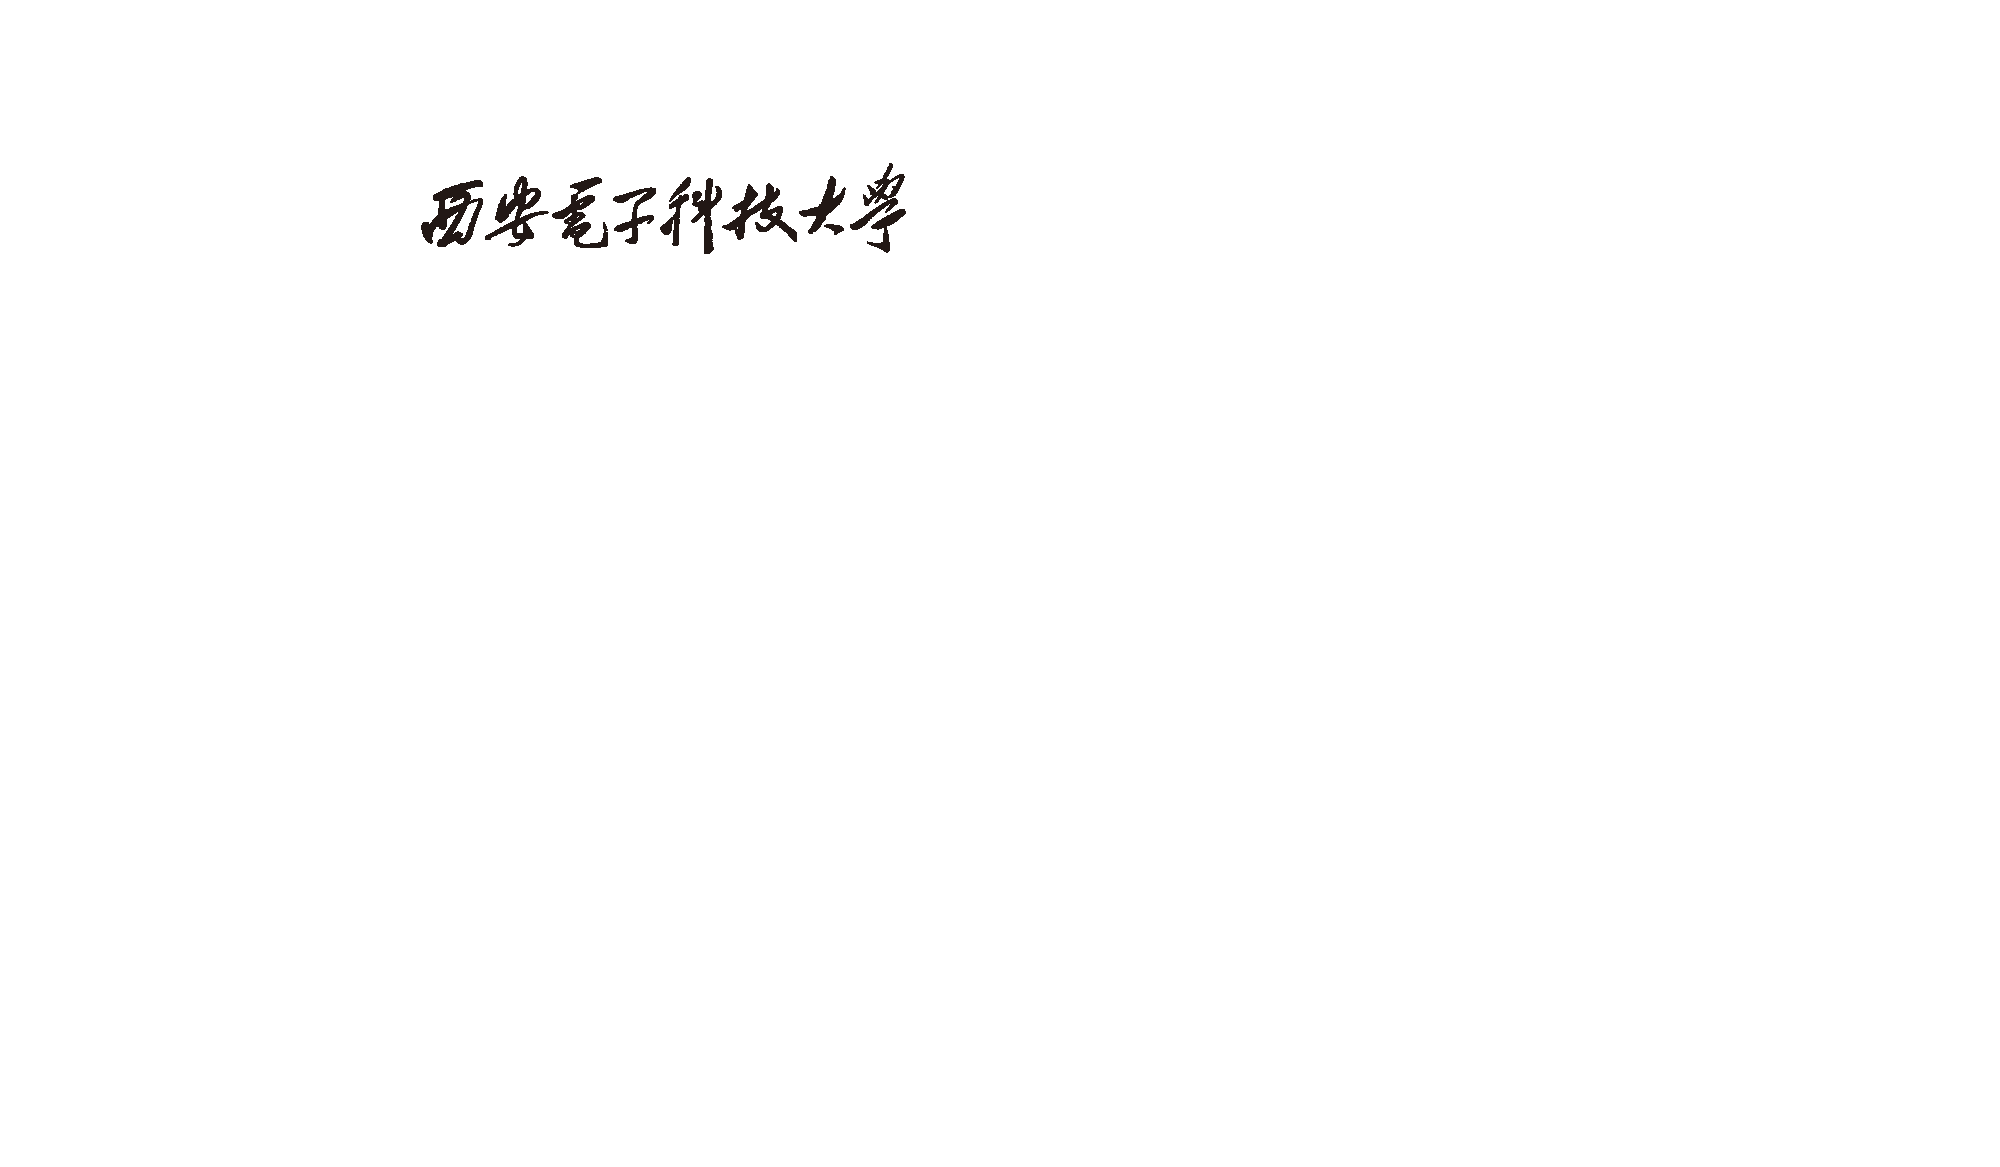
\includegraphics[width=0.5\textwidth]{./Figure/xidian.pdf}
  
  \vspace*{\stretch{2}}
  
  \begin{center}
  {\centering\heiti{\zihao{0}\XDU@subject}}
  \end{center}
  
  \vspace*{\stretch{3}}
  
  \begin{center}
  
\includegraphics[width=0.25\textwidth]{./Figure/logo.pdf}
  \end{center}
\fi
\else
\if@nologo
  \vspace*{\stretch{15}}
\else
  \centering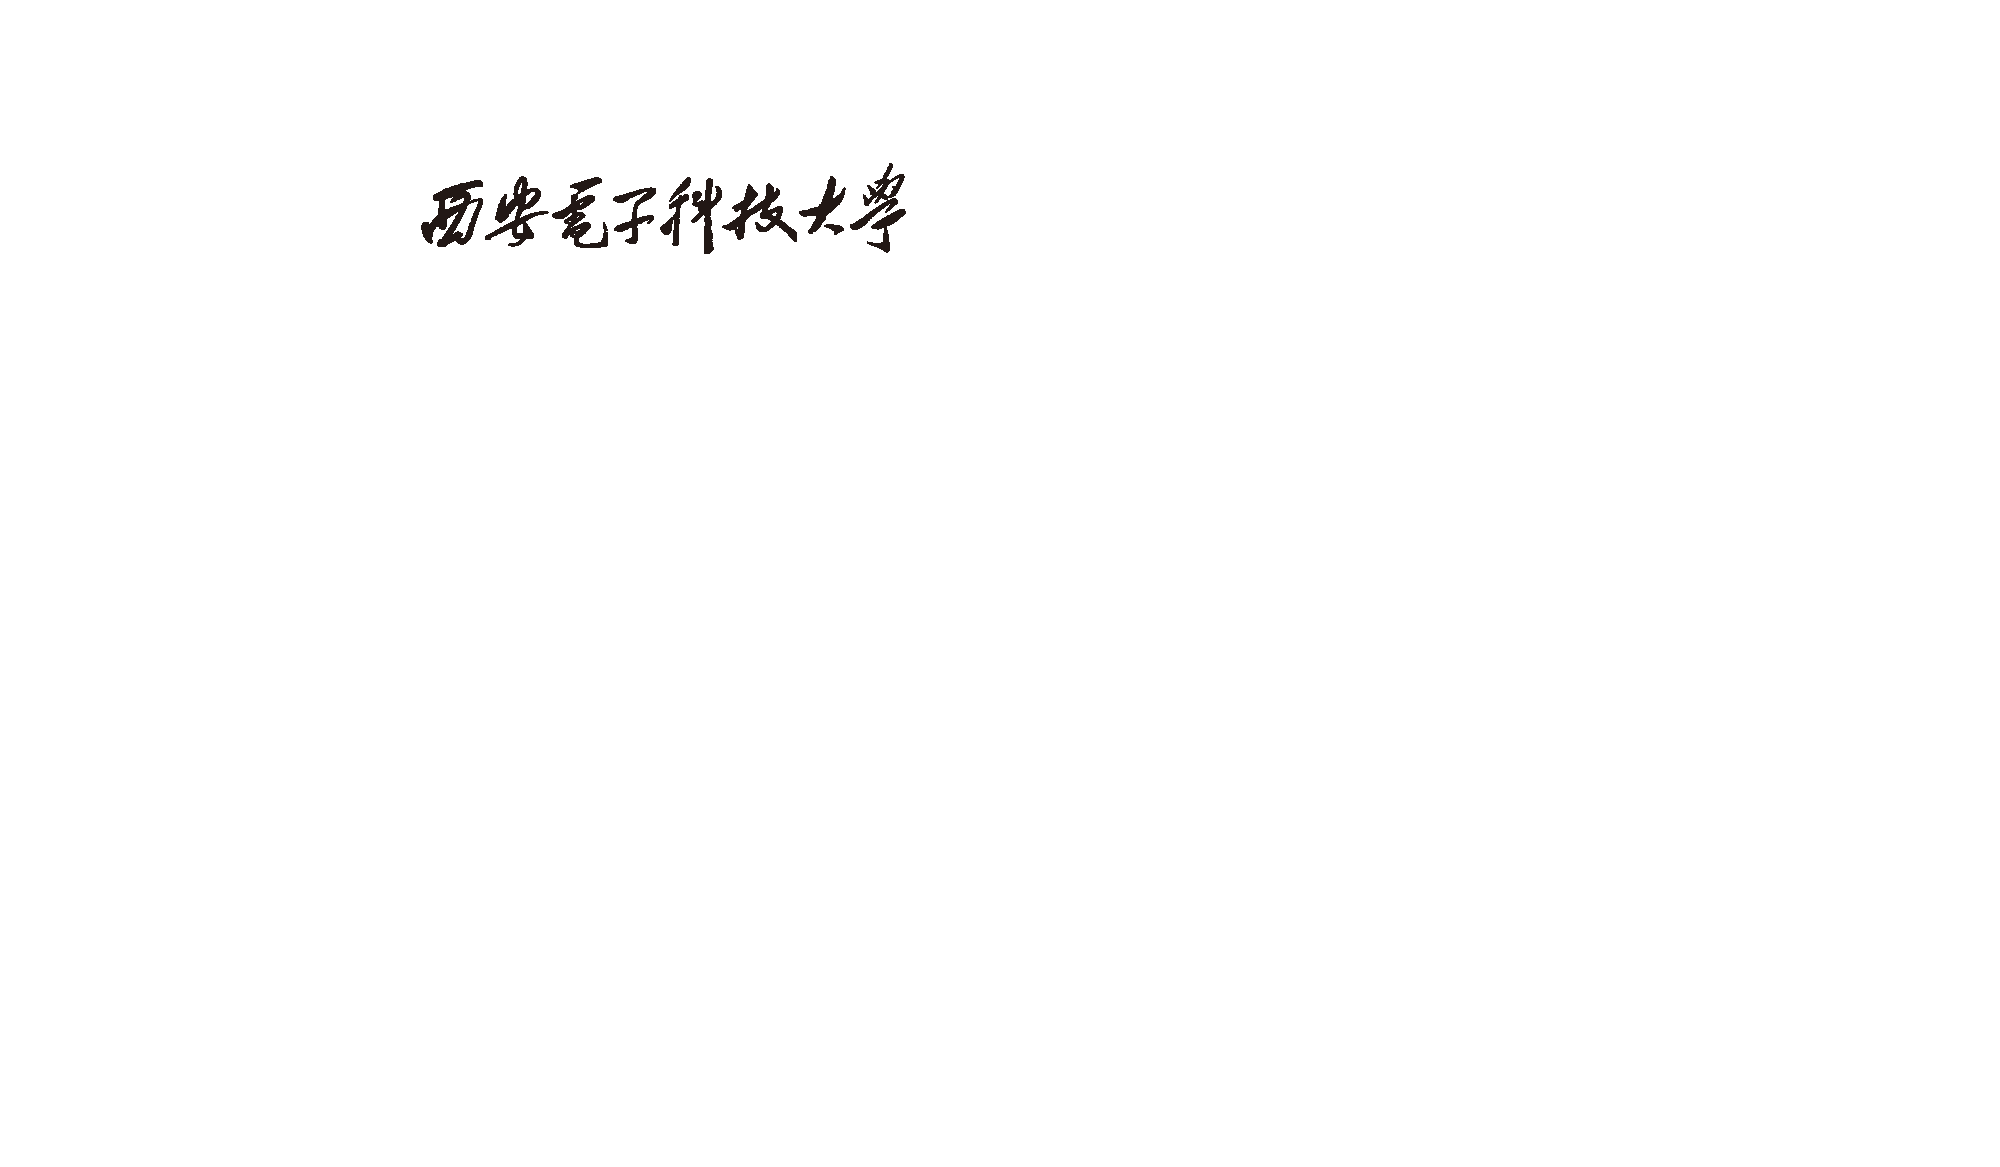
\includegraphics[width=0.5\textwidth]{./Figure/xidian.pdf}
  
  \vspace*{\stretch{4}}
  
  \begin{center}
  {\centering\heiti{\zihao{0}\XDU@subject}}
  \end{center}
  
  \vspace*{\stretch{5}}
  
  \begin{center}
  
\includegraphics[width=0.25\textwidth]{./Figure/logo.pdf}
  \end{center}
\fi
\fi

\vspace*{\stretch{4}}

\begin{center}
\begin{tabular}{c C{6.5cm}}
\textbf{\zihao{3}\XDU@titlename} & {\heiti\enheiti\zihao{3}\XDU@septitleA}\\
\cline{2-2}
 & \\
 & {\heiti\enheiti\zihao{3}\XDU@septitleB}\\
\cline{2-2}
 & \\
\textbf{\zihao{3}\XDU@schoolname} & {\zihao{-3}\XDU@school}\\
\cline{2-2}
 & \\
\textbf{\zihao{3}\XDU@majorname} & {\zihao{-3}\XDU@major}\\
\cline{2-2}
 &\\
\textbf{\zihao{3}\XDU@authorname} & {\zihao{-3}\XDU@author}\\
\cline{2-2}
 &\\
\textbf{\zihao{3}\XDU@supervisorname} & {\zihao{-3}\XDU@supervisor}\\
\cline{2-2}
\cline{2-2}
\end{tabular}
\end{center}

\end{titlepage}

\pagestyle{empty}
\cleardoublepage

\begin{center}
{\textbf{\zihao{1}\XDU@declarename}}
\end{center}

\vspace*{3em}

{\songti{\zihao{4}\XDU@declaretext}}

\vspace*{8em}

{\songti\zihao{4}\XDU@authornametitle\CJKunderline{\phantom{\qquad\qquad\qquad\quad}}%
\XDU@signedname\quad\XDU@timename\@date

\XDU@supervisorhasread\CJKunderline{\phantom{\qquad\qquad\quad}}%
\XDU@signedname\quad\XDU@timename\@date}

\make@abstract%

\frontmatter
\tableofcontents%
\mainmatter
}
%</cls>
%    \end{macrocode}
%
% \changes{v0.1}{2015/12/02}{对封面相关关键字进行配置}
% \changes{v0.1.3}{2016/02/23}{增加关键字定义,使得模板更加规范。}
%    \begin{macrocode}
%<*cfg>
%% 以下内容勿动
\subject{本科毕业设计论文}
\newcommand{\XDU@classname}{班\quad 级}
\newcommand{\XDU@schoolnumbername}{学\quad 号}
\newcommand{\XDU@titlename}{题\qquad 目}
\newcommand{\XDU@schoolname}{学\qquad 院}
\newcommand{\XDU@majorname}{专\qquad 业}
\newcommand{\XDU@authorname}{学生姓名}
\newcommand{\XDU@supervisorname}{导师姓名}
\newcommand{\XDU@declarename}{毕业设计(论文)诚信声明书}
\newcommand{\XDU@declaretext}{本人声明:本人所提交的毕业论文《\CJKunderline{\XDU@title}》是本人在指导教师指导下独立研究、写作成果,论文中所引用他人的无论以何种方式发布的文字、研究成果,均在论文中加以说明;
有关教师、同学和其他人员对本文本的写作、修订提出过并为我在论文中加以采纳的意见、建议,均已在我的致谢辞中加以说明并深致谢意。\par
本文和资料若有不实之处,本人承担一切相关责任。}


\newcommand{\XDU@authornametitle}{论文作者:}
\newcommand{\XDU@signedname}{(签字)}
\newcommand{\XDU@timename}{时间:}
\newcommand{\XDU@supervisorhasread}{指导教师已阅:}
%% 
%</cfg>
%    \end{macrocode}
%\end{macro}
%
% \subsection{代码环境}
%    \begin{macrocode}
%<*cls>
\ifxetex
  \lstset{
   showstringspaces=false,
   showspaces=false,
   tabsize=4,
   frame=lines,
   basicstyle = \XDU@codebasicfont,
   keywordstyle = \color{XDU@keywordcolor}\bfseries,
   stringstyle = \color{XDU@stringcolor}\ttfamily,
   commentstyle = \color{XDU@commentcolor}\rmfamily\itshape,
   identifierstyle=,
   columns = flexible,
   numbers = left,
   numberstyle = \footnotesize
  }
\else
  \lstset{
   showstringspaces=false,
   showspaces=false,
   tabsize=4,
   frame=lines,
   basicstyle = \XDU@codebasicfont,
   keywordstyle = \color{XDU@keywordcolor}\bfseries,
   stringstyle = \color{XDU@stringcolor}\ttfamily,
   commentstyle = \color{XDU@commentcolor}\rmfamily\itshape,
   identifierstyle=,
   columns = flexible,
   numbers = left,
   numberstyle = \footnotesize,
   extendedchars = false,
   escapechar = `
  }
\fi
\ifxetex
  \lstdefinestyle{nonumbers}
  {
   showstringspaces=false,
   showspaces=false,
   tabsize=4,
   frame=lines,
   basicstyle = \XDU@codebasicfont,
   keywordstyle = \color{XDU@keywordcolor}\bfseries,
   stringstyle = \color{XDU@stringcolor}\ttfamily,
   commentstyle = \color{XDU@commentcolor}\rmfamily\itshape,
   identifierstyle=,
   columns = flexible,
   numbers = none,
   numberstyle = \footnotesize
  }
\else
  \lstdefinestyle{nonumbers}
  {
   showstringspaces=false,
   showspaces=false,
   tabsize=4,
   frame=lines,
   basicstyle = \XDU@codebasicfont,
   keywordstyle = \color{XDU@keywordcolor}\bfseries,
   stringstyle = \color{XDU@stringcolor}\ttfamily,
   commentstyle = \color{XDU@commentcolor}\rmfamily\itshape,
   identifierstyle=,
   columns = flexible,
   numbers = none,
   numberstyle = \footnotesize,
   extendedchars = false,
   escapechar = `
  }
\fi
%    \end{macrocode}
%
% \subsection{致谢环境}
% 定义致谢环境,用于致谢一章;
%    \begin{macrocode}
\newenvironment{thanksfor}{\backmatter
\chapter{\XDU@thanksforname}}{\comtinuematter}
%    \end{macrocode}
%
% \subsection{其他细节}
% 声明宏命令,将论文中文关键词写入PDF文件
%\begin{macro}{\XDU@setpdf@keywords}
%    \begin{macrocode}
\def\XDU@setpdf@keywords{
    \hypersetup{
	    pdfkeywords={\XDU@keywords}
    }
}
%    \end{macrocode}
%\end{macro}
% 在文章开头导言区加入以下命令,设置最终生成的PDF属性;
%    \begin{macrocode}
\AtBeginDocument{
\hypersetup{
    pdftitle={\XDU@title},
    pdfauthor={\XDU@author},%
    pdfsubject={\XDU@subject},
    pdfcreator={\XDU@author},
    pdfproducer={XDUthesis}
}
}
%    \end{macrocode}
% 在文档类型最后,导入模板配置文件。
%    \begin{macrocode}
\AtEndOfClass{%%
%% This is file `XDUthesis.cfg',
%% generated with the docstrip utility.
%%
%% The original source files were:
%%
%% XDUthesis.dtx  (with options: `cfg')
%% 
%% This is a generated file.
%% 
%% Copyright (C) 2015--2019 by Stick Cui <Stick_Cui@163.com>
%% 
%% This file may be distributed and/or modified under the
%% conditions of the LaTeX Project Public License, either version 1.3c
%% of this license or (at your option) any later version.
%% The latest version of this license is in:
%% 
%% http://www.latex-project.org/lppl.txt
%% 
%% and version 1.3c or later is part of all distributions of LaTeX
%% version 2008/05/04 or later.
%% 
%% To produce the documentation run the original source files ending with `.dtx'
%% through LaTeX.
%% 

\ProvidesFile{XDUthesis.cfg}
[2019/05/11 0.1.9 Xidian University Thesis Template]
%% 摘要
\abstractname{摘\quad 要}
\enabstractname{Abstract}
\newcommand{\XDU@abstractnameheader}{摘要}
\newcommand{\XDU@contentsnameheader}{目录}
\newcommand{\XDU@keywordsname}{关键词}
\newcommand{\XDU@enkeywordsname}{Key words}
%% 关键词分隔符
\def\XDU@keywords@separator{\quad }
\def\XDU@enkeywords@separator{\quad }
%% 致谢一章的标题名
\thanksforname{致\quad 谢}
\thanksfornameheader{致谢}
%% 代码标题
\renewcommand\lstlistingname{代码}

%% 代码高亮颜色:如有需要修改rgb值即可
%% rgb = 0.7,0.2,0.2  西电视觉识别系统规定的红色
%% rgb = 0,0.25,0.51  西电视觉识别系统规定的蓝色
\definecolor{XDU@keywordcolor}{rgb}{0.7,0.2,0.2}%% 关键词颜色
\definecolor{XDU@stringcolor}{rgb}{0.84,0.62,0.52}%% 字符串颜色,仿Visual Studio默认配色
\definecolor{XDU@commentcolor}{rgb}{0.15,0.55,0.15}%% 注释的颜色,仿Visual Studio默认配色
%% 代码字体:这个字体族看着舒服,目前还不知道是否符合,论文规范
\def\XDU@codebasicfont{\fontfamily{pcr}\selectfont}

%% 以下内容勿动
\subject{本科毕业设计论文}
\newcommand{\XDU@classname}{班\quad 级}
\newcommand{\XDU@schoolnumbername}{学\quad 号}
\newcommand{\XDU@titlename}{题\qquad 目}
\newcommand{\XDU@schoolname}{学\qquad 院}
\newcommand{\XDU@majorname}{专\qquad 业}
\newcommand{\XDU@authorname}{学生姓名}
\newcommand{\XDU@supervisorname}{导师姓名}
\newcommand{\XDU@declarename}{毕业设计(论文)诚信声明书}
\newcommand{\XDU@declaretext}{本人声明:本人所提交的毕业论文《\CJKunderline{\XDU@title}》是本人在指导教师指导下独立研究、写作成果,论文中所引用他人的无论以何种方式发布的文字、研究成果,均在论文中加以说明;
有关教师、同学和其他人员对本文本的写作、修订提出过并为我在论文中加以采纳的意见、建议,均已在我的致谢辞中加以说明并深致谢意。\par
本文和资料若有不实之处,本人承担一切相关责任。}

\newcommand{\XDU@authornametitle}{论文作者:}
\newcommand{\XDU@signedname}{(签字)}
\newcommand{\XDU@timename}{时间:}
\newcommand{\XDU@supervisorhasread}{指导教师已阅:}
%%
%% 定理类声明:来自清华大学LaTeX模板
\theoremsymbol{\ensuremath{\square}}
\newtheorem*{proof}{证明}
\theoremstyle{plain}
\theoremsymbol{}
\theoremseparator{:}
\newtheorem{assumption}{假设}[chapter]
\newtheorem{proposition}{命题}[chapter]
\newtheorem{lemma}{引理}[chapter]
\newtheorem{theorem}{定理}[chapter]
\newtheorem{axiom}{公理}[chapter]
\newtheorem{corollary}{推论}[chapter]
\newtheorem{exercise}{练习}[chapter]
\newtheorem{example}{例}[chapter]
%\newtheorem{remark}{注释}[chapter]
\newtheorem{problem}{问题}[chapter]
\newtheorem{conjecture}{猜想}[chapter]
\newtheorem{definition}{定义}[chapter]
\newtheorem{convention}[definition]{惯例}
\newtheorem{property}[definition]{性质}
\newtheorem{transformation}[definition]{变换}
\newtheorem{remark}[definition]{注释}


%\newtheorem{convention}{惯例}[chapter]
%\newtheorem{property}{性质}[chapter]
%\newtheorem{transformation}{变换}[chapter]

%% 字体项,除非是正文字体不是规定的宋体,一般以下项目不需要
%% \setCJKmainfont[BoldFont={STZhongsong},ItalicFont={KaiTi}]{SimSun}
%% \setCJKsansfont[AutoFakeBold]{SimHei}
%% \setCJKmonofont{FangSong}
%% \setmainfont[NFSSFamily=entextrm]{Times New Roman}%
%% \setsansfont[NFSSFamily=entextsf]{Times New Roman}%
%%
%% 以下项目均为ctex默认设置,如无特殊需要,无须修改
 \ctexset{
  contentsname = {目\quad 录},
%%  listfigurename = {插图},%插图目录
%%  listtablename = {表格},%表格目录
%%  figurename = {图},
%%  tablename = {表},
%%  indexname = {索引},
%%  appendixname = {附录},
%%  bibname = {参考文献}
 }
%% 
%% This package consists of the file  XDUthesis.dtx,
%%              and the derived files XDUthesis.cls,
%%                                    XDUthesis.cfg.
%% 
%%
%% End of file `XDUthesis.cfg'.
}
%</cls>
%    \end{macrocode}
%
% \changes{v0.1}{2015/12/02}{其他配置}
% \changes{v0.1.8}{2019/04/17}{修改备用字体设置}
%    \begin{macrocode}
%<*cfg>
%% 定理类声明:来自清华大学LaTeX模板
\theoremsymbol{\ensuremath{\square}}
\newtheorem*{proof}{证明}
\theoremstyle{plain}
\theoremsymbol{}
\theoremseparator{:}
\newtheorem{assumption}{假设}[chapter]
\newtheorem{definition}{定义}[chapter]
\newtheorem{proposition}{命题}[chapter]
\newtheorem{lemma}{引理}[chapter]
\newtheorem{theorem}{定理}[chapter]
\newtheorem{axiom}{公理}[chapter]
\newtheorem{corollary}{推论}[chapter]
\newtheorem{exercise}{练习}[chapter]
\newtheorem{example}{例}[chapter]
\newtheorem{remark}{注释}[chapter]
\newtheorem{problem}{问题}[chapter]
\newtheorem{conjecture}{猜想}[chapter]
\newtheorem{convention}{惯例}[chapter]
\newtheorem{property}{性质}[chapter]
\newtheorem{transformation}{变换}[chapter]

%% 字体项,除非是正文字体不是规定的宋体,一般以下项目不需要
%% \setCJKmainfont[BoldFont={STZhongsong},ItalicFont={KaiTi}]{SimSun}
%% \setCJKsansfont[AutoFakeBold]{SimHei}
%% \setCJKmonofont{FangSong}
%% \setmainfont[NFSSFamily=entextrm]{Times New Roman}%
%% \setsansfont[NFSSFamily=entextsf]{Times New Roman}%
%% 
%% 以下项目均为ctex默认设置,如无特殊需要,无须修改
%% \ctexset{
%%  contentsname = {目录},
%%  listfigurename = {插图},%插图目录
%%  listtablename = {表格},%表格目录
%%  figurename = {图},
%%  tablename = {表},
%%  indexname = {索引},
%%  appendixname = {附录},
%%  bibname = {参考文献}
%% }
%</cfg>
%    \end{macrocode}
%
% \Finale
%
\endinput
% \iffalse
%  Local Variables:
%  mode: doctex
%  TeX-master: t
%  End:
% \fi